%!TEX root = main.tex
% \section{Solution - Hermes}
% \label{sec:solution}

\section{$\!\!\!$Hermes: Coinference-Centric LLM Serving$\!$}


\subsection{Overview}
\begin{figure}
    \vspace{-.1in}
    \centering
    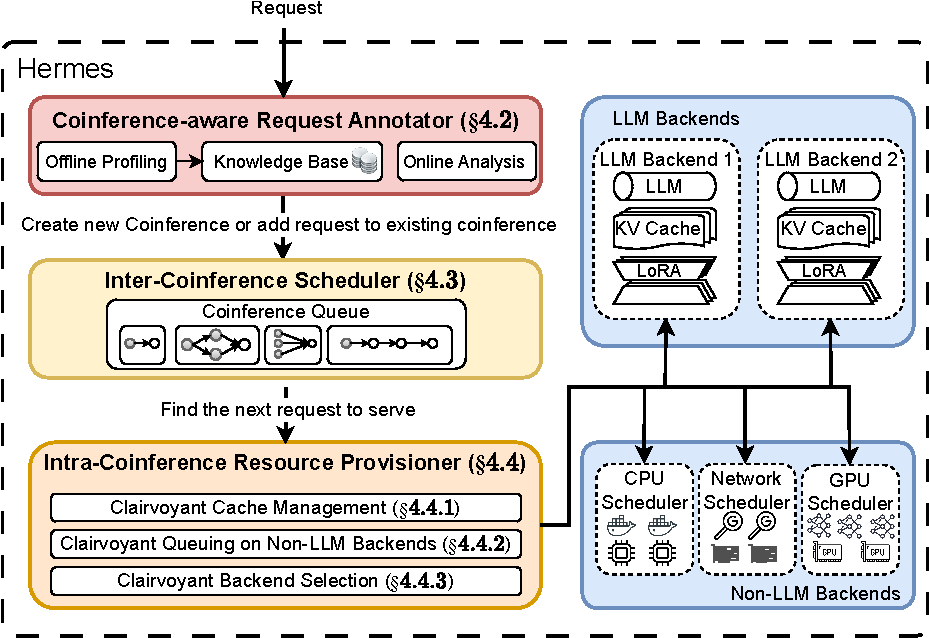
\includegraphics[width=0.95\linewidth]{figures/overview.drawio.pdf}
    \caption{The system architecture of Hermes.}
    \label{fig:overview}
    \vspace{-.2in}
\end{figure}

% Fig.~\ref{fig:overview} provides an overview of Hermes's design. Hermes incorporates a \emph{Coinference-aware Request Annotator} (\S\ref{subsec:demand_modeling}) to model the resource demand required to complete a Coinference. Each incoming request is added to a newly created or existing Coinference based on the information provided by the annotator. Besides, Hermes designs a Coinference-centric Scheduler called \emph{Inter-Coinference Scheduler} (\S\ref{subsec:inter-coinf scheduling}). This scheduler calculates the priority of each Coinference and allocates requests accordingly iteratively. Additionally, to enhance the service of high-priority Coinferences, Hermes includes an \emph{Intra-Coinference Resource Provisioner} (\S\ref{subsec:resource_provisioning}). This component ensures that Coinferences with higher priority receive better service, regardless of whether they involve LLM, Non-LLM, or multiple backend systems.

Based on the above coinference abstraction, in this paper we design Hermes, a coinference-centric serving system for LLM applications. 
Hermes has three key modules as shown in Fig.~\ref{fig:overview}.	
First, there is a \emph{Coinference-aware Request Annotator} (\S\ref{subsec:demand_modeling}) that annotates the coinference-level demand information for each incoming request, so as to facilitate later inter- and intra-application optimizations. 
The demand models are built offline with a series of profiling runs and stored in a knowledge base.
Second, the \emph{Inter-Coinference Scheduler} (\S\ref{subsec:inter-coinf scheduling}) determines the proper scheduling priority of different requests from the coinference-level viewpoint. 
Third, to efficiently execute each individual request, the \emph{Intra-Coinference Resource Provisioner} (\S\ref{subsec:resource_provisioning}) leverages the coinference-level demand information to prepare the desired resources in various aspects: cache management (\S\ref{subsubsec:cache}), queuing management on non-LLM backends (\S\ref{subsubsec:queuing}), and selection of LLM backends with different configurations (\S\ref{subsubsec:selection}). 


\begin{figure}
    \centering
    \begin{minted}[
    frame=none,
    obeytabs=true,
    framesep=0mm,
    baselinestretch=0.9,
    fontsize=\footnotesize,
    xleftmargin=0em,
    breaklines,
    texcomments,
    escapeinside=||
    ]{python}

"application-1":{
    "stage_list":[
        "stage-1":{
            "prompt_tokens": [500, 540,..., 510],
            "completion_tokens": [200, 250,..., 220],
            "request_parallelism": [3, 3,..., 3],
            "loop_times": [2,3,..., 4]
            "next_stage": "stage-2",
            "gap_to_next_stage": [1.2, 1.1, ..., 1.5],
            "demand_during_gap": {
                    "cpu_core": 1,
                    "memory": 2,
                },
            "demand_correlation_mask": (0,1,1,0,1),
        },
        "stage-2":...,
        "stage-3":...,
        ...
    ],
}

    \end{minted}
    \vspace{-0.3cm}
    \caption{An example of coinference demand model.} 
    %The Example of How We Model an Application \chen{describe the meaning?} \gz{For each application, we maintain a stage list that contains the information dictionary for every type of stage of this application. This information dictionary includes the distribution of resource demand (e.g. number of prompt tokens, number of output tokens), the probability of transitioning to every possible next stage, and a mask indicating demand correlation.}}
    \label{fig:demand_model}
\end{figure}


\subsection{Coinference Demand Modeling}
\label{subsec:demand_modeling}

In coinference demand modeling, we seek to panoramically capture the demand characteristics of an LLM application through a series of offline profiling runs. 
Our objective  here is to design a (1) \emph{general} representation method that is applicable to diverse LLM applications and, in the meantime, (2) as \emph{precise} as possible. 

\subsubsection{Towards general demand modeling.}
We first focus on the \emph{generality} aspect. 
To design a general demand modeling method, we need to properly handle the \emph{diversity} and \emph{uncertainty} of LLM applications. 
We will respectively show our solutions in such two aspects with Fig.~\ref{fig:demand_model}.

\textit{1) Handling structure and resource diversity.}
% First, different coinferences have their constituting LLM requests organized in different structures. 
% To be specific,
In typical LLM applications, there are heterogeneous relationships among the requests of a coinference: some requests are in parallel with each other,
%(e.g., for those in the summary-chunks phase in Fig.~\ref{fig:app_structure}(h)), 
whereas some others have rigid dependencies. % (e.g, for those across the generate and score phases in Fig.~\ref{fig:app_structure}(c)).  
To describe such diverse request relationships in a general manner, we adopt a \emph{stage-centric} paradigm.
An LLM application usually contains a series of functional units---each issuing one or multiple parallel inferences that are submitted almost concurrently and also share the \emph{same system prompt}; such a functional unit is defined as a \emph{stage}\footnote{
    The stage affiliation of a request can be manually annotated by the \texttt{extra\_body} parameter (as the application affiliation) or automatically detected by analyzing the prompt prefix.
}.
%At online serving time, the stage affiliation of a request can be easily identified from its prompt.} 
Therefore, we can organize the requests of a LLM application as a list of stages; each stage records the request-level demand (input/output token length) and also maintains a \texttt{next\_stage} property to record the dependency information.
% As shown in Fig.~\ref{fig:demand_model}, each stage maintains the \texttt{next\_stage} property to record the dependency information. 
% \chen{and we sketch the LLM resource demand (prompt token, completion token, parallism) based on the constituting requests.}
Second, executing an LLM application also requires diverse resource backends like CPU and network (for tool calling); such non-LLM resources are usually consumed  during the gaps between LLM inferences.
To express such non-LLM resource demand, we incorporate the consumption amount (e.g., 1 cpu core and 2GB memory) as well as the gap length to the dependency information, as expressed by the \texttt{gap\_to\_next\_stage}\footnote{
For LLM applications without tool calling (e.g., for Chatbot), \texttt{gap\_to\_next\_stage} can also be leveraged to represent the typical interaction pace incurred by factors like network transmission delay. 
} and \texttt{demand\_during\_gap} properties in Fig.~\ref{fig:demand_model}.

\textit{2) Handling structure and request-level uncertainty.}
Demand uncertainty (i.e., runtime dynamicity) means that an LLM application has different stage structures or demand quantities in different execution rounds.
% that the demand pattern of an LLM application usually fluctuates across different execution rounds, which may occur in various aspects: the stage structure,
%(for applications with ReActing and LLM-planning), 
%the request parallelism,
%(if not predefined but determined by inputs), 
%as well as the request input/output token length.
% Such variations need to be comprehensively expressed to facilitate future demand prediction.
Structural uncertainty is mainly caused by the looping LLM requests in ReActing-like applications\footnote{
We admit that plan-and-execute applications may also yield dynamic structures, which is difficult to address given the diverse functional units after planning. 
For consistent modeling with reasonably good performance, we dictate that each plan-and-execute application always has two stages---a \emph{planning} stage and an \emph{executing} stage. % , which can facilitate consistent modeling with reasonable good performance. 
In that sense, a N-step-after-planning application would have an \emph{executing} stage that loops for N times. 
}.
To build a stable application structure despite such looping dynamicity, we introduce the \texttt{loop\_times} property in each stage to describe its looping status across different profiling rounds.
Moreover, when expressing the quantity variation in each demand aspect (input/output token length, request parallelism, loop times and post-stage gap), we choose to 
%To express stage structure variation, we resort to a \emph{probability-graph-like} strategy: given that a stage may have multiple downstream branches (sometimes may looping to itself), we associate a \texttt{frequency} property to each downstream stage. 
% To express request parallelism variation, we choose to 
directly append the raw value profiled from each trial run to a list. 
We note that recording the raw values is better than recording the coefficients of the fitted skewed norm distribution, considering the depiction fidelity (the true distribution is in fact irregular) and computation efficiency---it takes much time (up to seconds) to fit out the coefficients as well as to support our later calculations (e.g., correlation analysis and integral calculus).
In practice, we set the maximal length of the recorded value list to $500$ (evicted in FIFO manner), and the storage cost is indeed negligible on cutting-edge GPU servers. 
% (fitting ou\footnote{
%     %We note that recording the raw values is better than recording the coefficients of the fitted skewed norm distribution shown in Fig.~\ref{fig:token_usage}: although the later is more concise, it is however not appropriate for our use.
%     First, there are still error gaps between the true distribution and the skewed norm distribution;
%     second, such an analytic method is not computation-efficient---it takes much time (up to seconds) to fit out the coefficients as well as to support our later calculations (e.g., correlation analysis and integral calculus).
%     %and applying them for our later integral operations (Sec. X) are computation-inefficient---taking even seconds with the \chen{XX lib}. 
%     In contrast, recording the raw data is computation-efficient, and the storage cost (we set a maximal record number $500$) is indeed negligible on cutting-edge GPU servers. 
% }.
% To express input/output length variation, we also record the raw data in a list. 
%Note that we additionally record the inter-stage time gaps---which may also vary across different rounds---in the same manner with raw data stored in list. 
%Moreover, we also record the execution time of the entire LLM application by summing up all the stage durations and gaps.
%\chen{some details unclear: multiple request? how to use mean and deviation?}

% \begin{figure*}
% 	\parbox[t]{18cm}{
% 		\centering
% 		{	
% 			\centering
% 			
\includegraphics[width=3.2cm]{figures/gap/1.pdf}
% 			\label{fig:gap_factoolkbqa}
% 		}\hfill
% 		{	
% 			\centering
% 			
\includegraphics[width=3.2cm]{figures/gap/4.pdf}
% 			\label{fig:gap_gotdocmerge}
% 		}\hfill
% 		{	
% 			\centering
% 			
\includegraphics[width=3.2cm]{figures/gap/2.pdf}
% 			\label{fig:gap_reactfever}
% 		}\hfill
% 		{	
% 			\centering
% 			
\includegraphics[width=3.2cm]{figures/gap/3.pdf}
% 			\label{fig:gap_reactalfw}
% 		}\hfill
% 		{	
% 			\centering
% 			
\includegraphics[width=3.2cm]{figures/gap/5.pdf}
% 			\label{fig:gap_langchainmapreduce}
% 		}\hfill
% 		{
% 			\centering
% 			
\includegraphics[width=3.2cm]{figures/duration/2.pdf}
% 			\label{fig:duration_factoolkbqa}
% 		}\hfill
% 		{	
% 			\centering
% 			
\includegraphics[width=3.2cm]{figures/duration/1.pdf}
% 			\label{fig:duration_gotdecmerge}
% 		}\hfill
% 		{	
% 			\centering
% 			
\includegraphics[width=3.2cm]{figures/duration/4.pdf}
% 			\label{fig:duration_reactfever}
% 		}\hfill
% 		{	
% 			\centering
% 			
\includegraphics[width=3.2cm]{figures/duration/5.pdf}
% 			\label{fig:duration_reactalfw}
% 		}\hfill
% 		{	
% 			\centering
% 			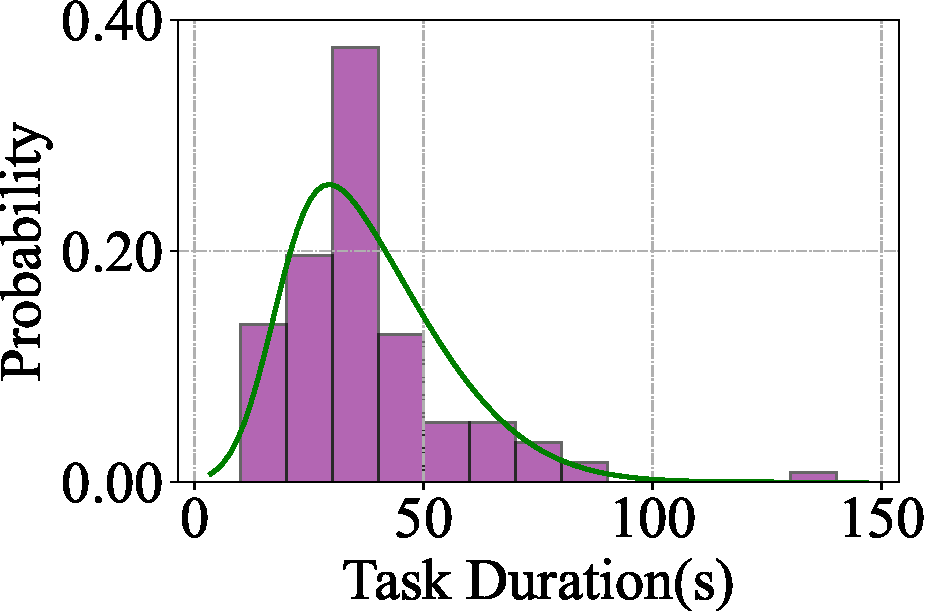
\includegraphics[width=3.2cm]{figures/duration/6.pdf}
% 			\label{fig:duration_langchainmapreduce}
% 		}\hfill
% 		\subfloat[FacTool kbqa]
% 		{
% 			\centering
% 			
\includegraphics[width=3.2cm]{figures/requestnum/0.pdf}
% 			\label{fig:requestnum_factoolkbqa}
% 		}\hfill
% 		\subfloat[GoT docmerge]
% 		{	
% 			\centering
% 			
\includegraphics[width=3.2cm]{figures/requestnum/5.pdf}
% 			\label{fig:requestnum_factoolmath}
% 		}\hfill
% 		\subfloat[ReAct fever]
% 		{	
% 			\centering
% 			
\includegraphics[width=3.2cm]{figures/requestnum/2.pdf}
% 			\label{fig:requestnum_reactfever}
% 		}\hfill
% 		\subfloat[ReAct alfw]
% 		{	
% 			\centering
% 			
\includegraphics[width=3.2cm]{figures/requestnum/3.pdf}
% 			\label{fig:requestnum_reactalfw}
% 		}\hfill
% 		\subfloat[LangChain mapreduce]
% 		{	
% 			\centering
% 			
\includegraphics[width=3.2cm]{figures/requestnum/4.pdf}
% 			\label{fig:requestnum_langchainmapreduce}
% 		}
% 		\caption{Gap Time, Task Duration and Number of Requests in Applications.}
% 		\label{fig:request_num}
% 	}
% \end{figure*}


% We are committed to developing a demand representation method for general LLM applications, capable of providing a comprehensive view of the app's execution process. By "comprehensive," we mean having a sufficient understanding of the app's requirements at both the coinference and stage levels, enabling effective coinference-level scheduling and resource provisioning.
% To achieve the above goal, we plan to approach Coinference Demand Modeling from two aspects: structure and demand.

% However, the greatest challenge lies in how to guarantee the precision and generality of the model when the modeling object is dynamical.
% The dynamics in structure primarily is because: within coinference, some stages exhibit dynamic changes in parallelism, and there are conditional jumps between stages, leading to structures such as loops and branches. Additionally, different coinferences may have significantly different structures due to design variations, as shown in Figure 1. With the ongoing development of LLM applications, even more diverse structures are expected to emerge.
% In terms of resource demands, the differences are even more pronounced. For LLM stages, we cannot know the length of decoding for each request, and the inputs and outputs of each stage are interrelated, making the execution process of coinference highly uncertain. In non-LLM stages, there may be calls to an expanding array of tools, which in turn rely on various traditional backend resources such as CPU and network bandwidth.
% Our goal is to include both existing and future potential structures and demands in our modeling framework, but this presents significant challenges.
% \subsubsection{Modeling for General and Complex Structure}


% To better harness LLM's potential in text analysis, problem-solving, and related areas, there is a growing trend toward dividing a complex application into what we call \textbf{Stages}, in which multiple LLM inferences are conducted with different prompts and Tools(like python, wiki...) are used to help generate LLM prompts containing different implications. This method succeed in improving LLM's performance, especially in complex application. We 
%  divide these applications that triggers multiple LLM inference into three categories according to structure pattern, and carry out a survey on demand aspects, which will be shown at 3.? in details.

% \textbf{Static Pipeline \& Static Parallelism:} in this kind of structure patterns,  the conduct order of stages and the parallelism of LLM requests in each stage are static. We take Factool\_code, Got\_docmerge for examples.   

% Factool\_code is an application provided by Factool to examine the factuality of the code generated for corresponding question. As shown in \ref{fig:factool_code_structure}, given the question and code answer, we first request LLM service to got several testcases, then we use LLM to generate another 3 solutions to the given question, after execute all the 4 solutions using python tool, we compare the result we get, if consistent, the code is factual.


% Got\_deocmerge is an application provided by Got to merge four documents into one. As shown in fig??, Got define a graph of operations, in which nodes represent the current state, while edges represent operations, so pipeline is static. The out-degree represent the parallelism of corresponding operation, whether using LLM or not, which is static too. With a stack-like controller, got is conduct in BFS order. 

% % First, we generate 5 possible result originating from initial state, then score them with the help of LLM and keep the best 3, after that we combine the best 3 in stage aggregate and generate 5 new node, score again and  only keep the best 1, originating from that generate 10 solutions, select the best as result.

% \textbf{Static Pipeline \& Dynamic Parallelism:} in the kind of structure pattern, pipeline is also static, but in some stages the parallelism of LLM requests varies between Coinferences. We take Factool\_kbqa, Factool\_math for example.

% Factool\_kbqa is an application in Factool to examine the factuality of a question-answer pair. As shown in fig??, we first ask LLM to conclude all claims contained in the answer, then generate particular queries that could justify the turth of each claim, therefore the parallelism of the stage query\_generation is up to how many claims attained in stage claim\_generation, which varies when input changes. For each query, we search it on wiki, this stage demand no LLM resource and lead into gap between LLM inference. In verify stage, we ask LLM to distinguish whether the wiki-search result support the corresponding claim, the parallelism of this stage is consistent with stage query\_generation. If all claims supported, the question-answer pair is factual.

% Factool\_math is similar to Factool\_kbqa, while in Factool\_math, inputs are math problem and its answer, claims represent every  calculate in the answer, queries are pieces of python code which could do the calculates in claims, after execute python calculate instead of wiki search, we could verify the truth of each claim without LLM in this application. The parallelism of stage query\_generation is dynamic, because the num of claims is not sure.  

% \textbf{Dynamic Pipeline:} in this kind of structure pattern, some stage's 
% successor have more than one selections, so they don't have fixed pipeline with single direction. Stages' parallelism could be dynamic too theoretically, but not usual in current applications. We take react\_fever, react\_alfw for examples.

% React\_fever and React\_alfw are applications of react in FEVER (Fact Extraction and Verification) and ALFWorld (Action Learning From the Web). As shown in fig??, stages alternate between think and action, the environment take actions guided by LLM response in think stage, return the observation (google-search result in React\_fever or text-world changes in React\_alfw), which will be added into prompt of next think stage.

% In all applications above, users are mainly concerned about the whole conduct time instead of time duaration of each single stage. We conduct measurements on both whole task time and stages' demand, table?? show their type and range of the dataset. fig?? show the task\_time distribution of different applications, the difference between them make it possible to predict and perform SJF scheduling.

% \begin{table}[htbp]
%     \centering
%     \begin{tabular}{|c|c|c|c| }
%         \hline
%         application & Pipeline & parallelism & size of dataset \\ \hline
%         Factool\_code & Static  & Static  & 164 \\ \hline
%         Got\_docmerge & Static & Static  & 100 \\ \hline
%         Factool\_kbqa & Static & Dynamic & 256 \\ \hline
%         Factool\_math & Static & Dynamic & 100 \\ \hline
%         React\_fever & Dynamic & Static & 105 \\ \hline
%         React\_alfw & Dynamic & Static & 95\\ \hline
%         Mapreduce & Dynamic & Dynamic & 112 \\ \hline
%     \end{tabular}
%     \caption{basic information of applications under conduct}
%     \label{tab:agent_list}
% \end{table}

% \begin{figure}[htbp]
%     \centering
%     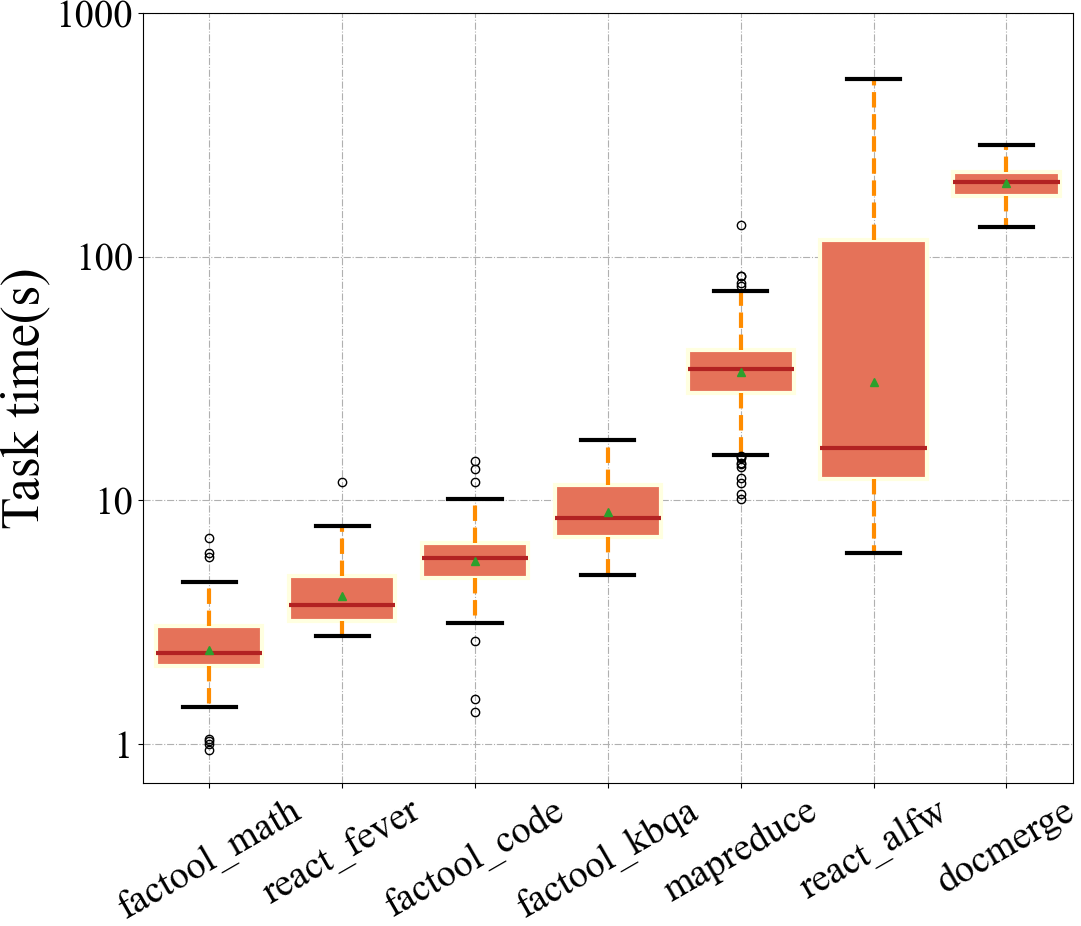
\includegraphics[width=\linewidth]{figures/box.png}
%     \caption{The box plot of coinference time of applications}
%     \label{fig:time_task_all}
% \end{figure}


% \subsubsection{Modeling for Rich and Scalable Attributes}

% \yfliu{During the life cycle of a coinfer, it can be in one of three states: UnFinished, Stage-Finished, or Coinference-Finished.}

% \begin{figure}[t]
%     \centering
%     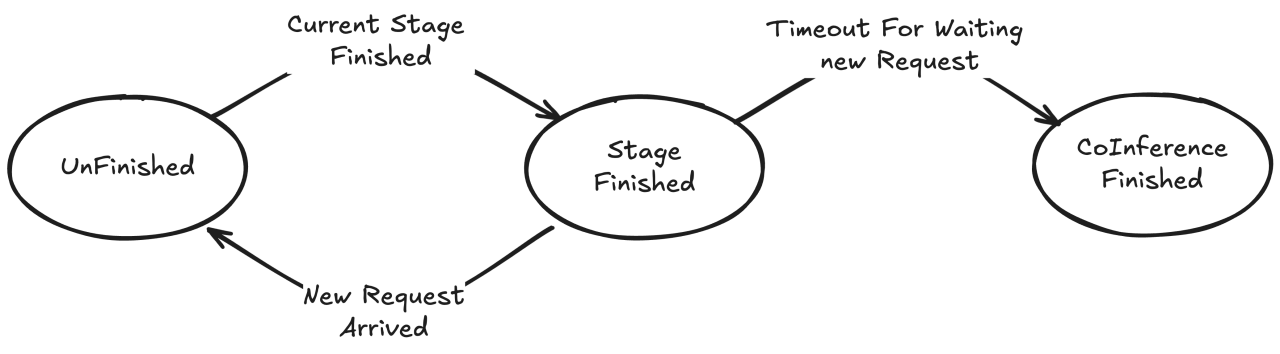
\includegraphics[width=1\linewidth]{figures/state_machine.png}
%     \caption{state machine}
%     \label{fig:state_machine}
% \end{figure}

% We use histograms to describe the distribution of various stage attributes, such as gap duration, number of parallel requests, prompt length, output length, and the transition probabilities to next stages (mainly the times it may loop).

\subsubsection{Towards precise demand modeling.}
\label{subsubsec:correlation_analysis}

Note that the ultimate purpose of demand modeling is to support accurate demand prediction at runtime. 
So far, we have made that by creating a general stage demand portrait from the past execution rounds.
Apart from such cross-round hints, we can future enhance the prediction accuracy by correlation hints in the ongoing round.
Due to the structural dependencies among stages, the resource demands of a stage are often correlated to the upstream ones. 
We note that there typically exist three cross-stage\footnote{
    For simplicity, we assume a Markov model in correlation analysis and only consider the correlation between directly dependent stages.
    }
demand correlation patterns:

    \emph{1)} A stage's request input length may be correlated to the upstream stage's request input length and output length.
        For example, for the Document Merging application, the input of each request in the \emph{scoring} stage is a superset of a request's output in the (upstream) \emph{aggregate} stage (plus a fixed system prompt). 
        Meanwhile, for the looping stages, downstream requests would share the same prompt template as the upstream ones, indicating similarity in input length.
    \emph{2)} A stage's request output length may be correlated to its input length as well as the upstream stage's request output length.
	% Note that the input and output length might be correlated in some cases.
	For example, for the \emph{generate-code} stage in Code Checking application, a more complex input task (often with a longer prompt) usually yields a longer code segment; so for other LLM-tasks like translation and article correction/polishing.
	Meanwhile, for the looping states, the request output lengths are also similar across stages.
    \emph{3)} A stage's request parallelism may be correlated to the upstream stage's request parallelism. 
	For example, as shown in KBQAV applications, for each inference request in the (upstream) \emph{generate-queries} stage, a corresponding inference request would be launched at the (downstream) \emph{verify-claim} stage.

\begin{figure}[t]
	\centering
	\vspace{-0.1in}

    \subfloat[KBQAV]
    {	
        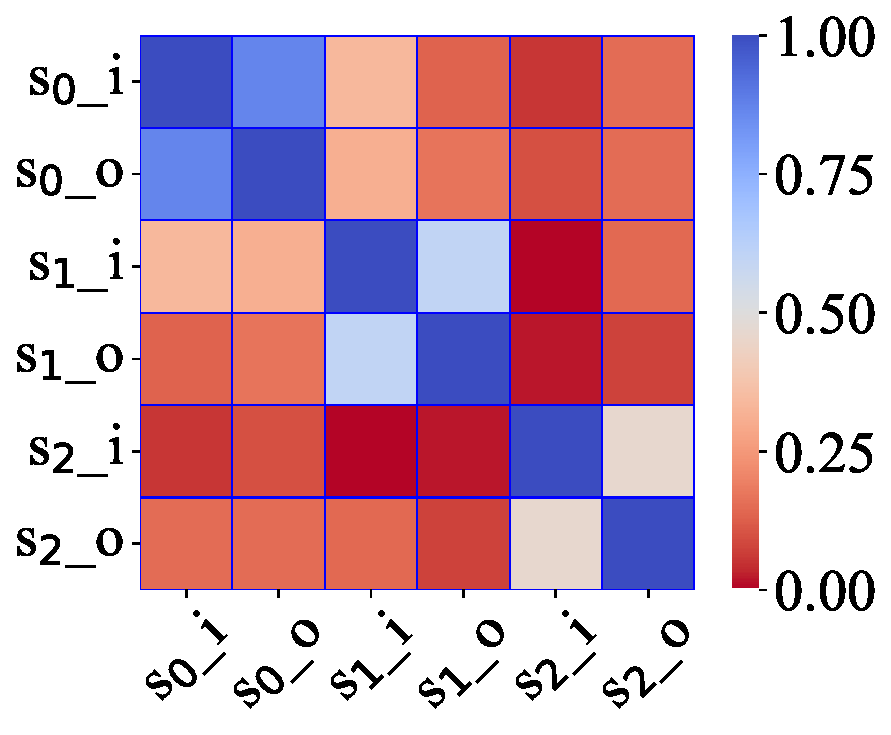
\includegraphics[width=0.45\linewidth]{figures/heatmap_kbqa.pdf}
        \label{fig:heatmap_kbqa}
    }  
    % \subfloat[Math\_FacTool]
    % {	
    %     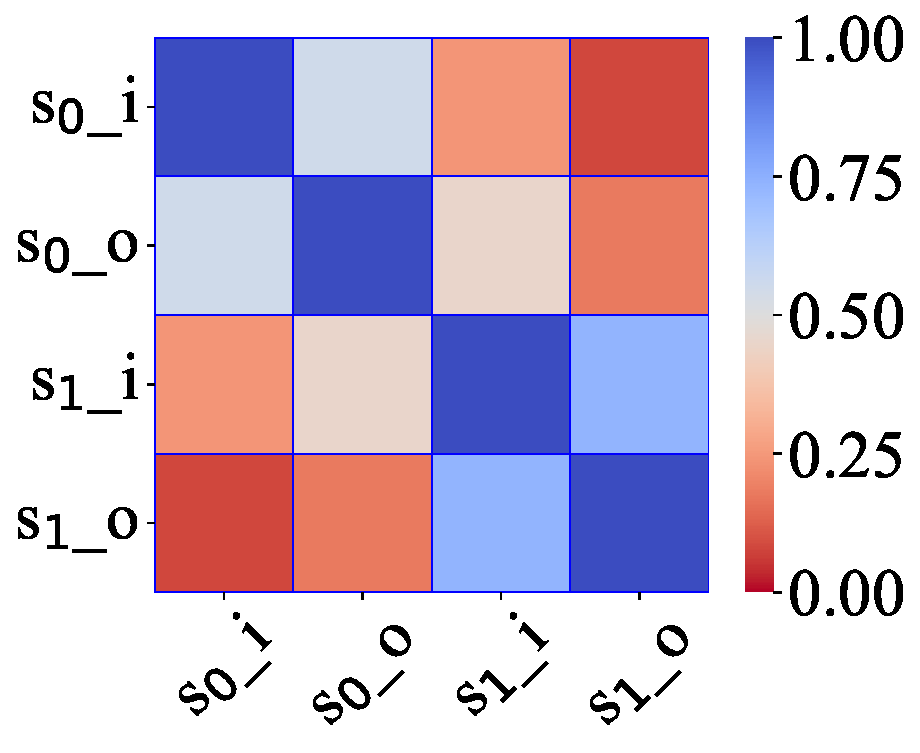
\includegraphics[width=0.2\linewidth]{figures/heatmap_math.pdf}
    %     \label{fig:heatmap_math}
    % }
    \subfloat[Document Merging (DM)]
    {
        \label{fig:heatmap_docmerge}
        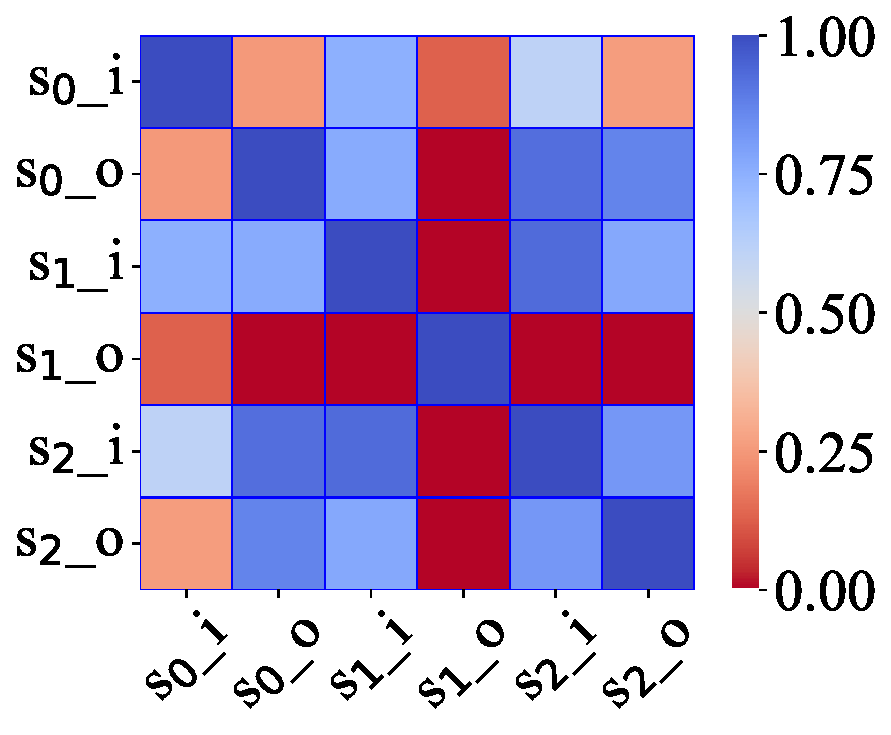
\includegraphics[width=0.45\linewidth]{figures/heatmap_mapreduce.pdf}
    }    
	\vspace{-0.05in}
	\caption{The Pearson correlation coefficients between input/output token lengths of different stages. We present the first three stages of KBQAV and DM, where $s_x$\_$i$ and $s_x$\_$o$ represent the input and output token length of the $x$-th stage.
        }
	\vspace{-0.1in}
	\label{fig:heatmap}
\end{figure}

To verify the existence of above correlation types (especially the first two), we resort to Pearson Correlation Analysis~\cite{sedgwick2012pearson} based on our profiled data over 100 trial runs.
We also divide the demand range to 10 buckets (as in Fig.~\ref{fig:token_usage} for ease of analysis), and use $P(X=i) (i=0,1,…,9)$ to represent the probability that the demand quantity variable X falls into bucket-$i$.
Then we calculate the Pearson correlation coefficient between two demand variables X and Y as
% Although modeling revealed that the input and output lengths of LLM requests approximate a skewed distribution, tending to cluster around the mean, the above experiments indicate that relying solely on the offline profile's mean is insufficient to achieve satisfactory prediction accuracy. Therefore, we aim to incorporate an online updating mechanism. Additionally, during the experiments, it was observed that the input and output lengths of different stages are directly or indirectly related. For instance, in React-style tasks, the output from one stage is directly added to the input of the next, leading to a growth trend in inputs. Similarly, in document merge tasks, longer inputs at the beginning often result in longer inputs and outputs in subsequent stages. We measured the correlation between stages of two applications using the Pearson correlation coefficient and represented it with the heatmap Figure \ref{fig:heatmap}. From the visualization results, it is evident that there is indeed a correlation between the inputs and outputs of certain stages within the app. Thus, we introduce Bayesian networks to learn such relationships. 
$\rho_{X,Y} = \frac{\text{cov}(X,Y)}{\sigma_X \sigma_Y} = \frac{\mathbb{E}((X - \mu_X)(Y - \mu_Y))}{\sigma_X \sigma_Y}.$	
In Fig.~\ref{fig:heatmap}, for KBQAV and Document Merging, we further depict the Pearson correlation coefficients between any two demand variables (each represent the input/output length of a stage).
For KBQAV, each stage's output length is strongly correlated to its input length; yet for Document Merging, each stage's input length is highly-related to the upstream stage's input length. 
Fig.~\ref{fig:heatmap} also suggests that each application has distinct correlation patterns; for prediction efficiency, we only consider the demand correlations with a coefficient ($\rho$) larger than 0.5.
To that end, in each stage we add a five-tuple $({M_I^\tilde{I}}, {M_I^\tilde{O}}, {M_O^\tilde{O}}, {M_O^I}, {M_P^\tilde{P}})$ to mask whether the corresponded demand correlation holds: $M_B^A$ represents whether the demand variable $A$ affects $B$; $I$, $O$ and $P$ ($\tilde{I}$, $\tilde{O}$ and $\tilde{P}$) respectively represents the input length, output length and request parallelism of the current (upstream) stage.

The above correlation analysis enables more precise online demand prediction.
Upon the completion of a stage, its execution information can be immediately adopted for demand prediction of the next stage. 
In that case, we are facing a \emph{conditional prediction} problem.
Suppose the request input and output length of the just-finished stage is respectively in bucket $i$ and $o$---with both correlated with the input length of the downstream stage, and we need to predict $P(I|\tilde{I}=I, \tilde{O}=o)$. 
To accomplish that, we join the historical execution records of the two stages (i.e., yielding $(\tilde{I}, \tilde{O}, I)$ tuples respectively from each trial round), and filter out the profiled tuples satisfying $\tilde{I}=i$ and $\tilde{O}=o$; then the $I$ distribution within the filtered records is a more precise prediction for the current round.

% For applications with a Directed Acyclic Graph (DAG) structure, we model each stage’s inputs and outputs across consecutive stages and establish links between each stage and its subsequent stages, forming a Bayesian network for inference. As co-inference proceeds, we sequentially obtain information from each stage, which allows us to make continuously refined predictions for the subsequent stages.Let $ \mathbf{X}_1, \mathbf{X}_2, \dots, \mathbf{X}_n $ be the random variables representing each stage in an application and $ \mathbf{X}_\text{prev} = \{ \mathbf{X}_1, \mathbf{X}_2, \dots, \mathbf{X}_{k-1} \} $ be the variables prior to stage $\mathbf{X}_k$, $ x_\text{prev} = \{ x_1, x_2, \dots,x_{k-1} \}$ presents execution information from previous stages. The conditional probability distribution(CPD) could be represented as equation \ref{eq:bayes cpd}. 

% \begin{equation}
%     P_\text{app}(X_h \mid \mathbf{X}_{\text{prev}} = x_{\text{prev}}) \quad k\leq h\leq n 
% \label{eq:bayes cpd}
% \end{equation}

% For non-DAG applications, especially those with cyclic units, we internalize the concepts of Bayesian maximum likelihood and probability updating. During online execution, we incorporate the encountered input and output results into the offline collected samples and use maximum likelihood methods to predict potential values of the next stage.Let $\{ x_k^{(0)},x_k^{(1)},\dots,x_k^{(m)}\}$represent all possible values of $\mathbf{X}_k$ after discretization. Let $P_{\text{init}}$ and $P_{\text{updated}}$ represent the initial distribution and the updated distribution, respectively. $\mathbf{X}_k = x_k^{(\text{obs})}$ represents the actual observed result for stage $\mathbf{X}_k$. Equation \ref{eq:cpd updated}, \ref{eq:cpd normalize} illustrates how the probability distribution is updated in response to the observed values.

% \begin{multline}
%     P_{\text{updated}}(\mathbf{X}_k = x_k^{(i)}) = (1 - w) P_{\text{init}}(\mathbf{X}_k = x_k^{(i)}) \\
%     + w \cdot \mathbf{sgn}(x_k^{(i)} = x_k^{(\text{obs})})    
% \label{eq:cpd updated}
% \end{multline}

% \begin{multline}
%     P_{\text{updated}}(X_k = x_k^{(i)}) \leftarrow \frac{P_{\text{updated}}(X_k = x_k^{(i)})}{\sum_{j} P_{\text{updated}}(X_k = x_k^{(j)})}
% \label{eq:cpd normalize}
% \end{multline}

% Based on the probability distribution adjusted by the execution results, we can predict the information of following stages more exactly. Due to our two methods, our prediction becomes applicable to a broader and more general range of scenarios. Figure \ref{fig:bayes effect} illustrates the results after adding Bayesian predictions.
% \begin{figure}[htbp]
%     \centering
%     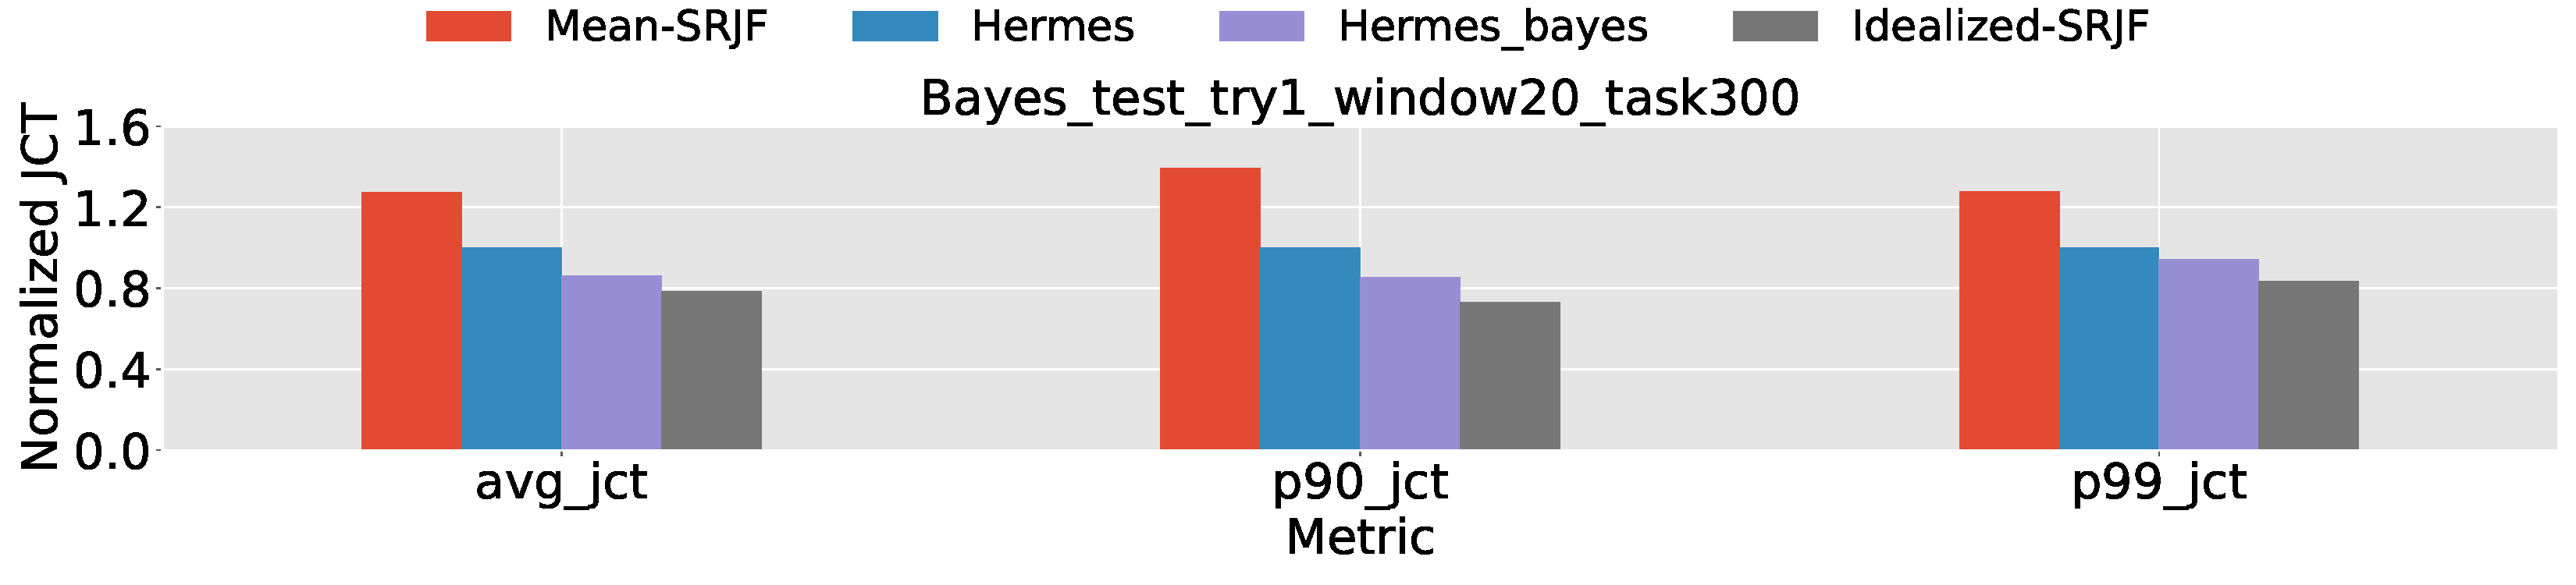
\includegraphics[width=\linewidth]{figures/bayes_mean.pdf}
%     \caption{Comparison of overall execution performance differences across various prediction methods.}
%     \label{fig:bayes effect}
% \end{figure}


\subsection{Inter-Coinference Scheduling}
\label{subsec:inter-coinf scheduling}

As previously showed in Fig.~\ref{fig:toy_example}, the conference abstraction provides us with a high-level scheduling handle.
%  which can effectively support high-level scheduling objectives.  
In this part, we explore how to leverage the coinference modeling results to optimize the inter-coinference scheduling performance.
There are two specific challenges. 
First, how to leverage the distribution-style demand description for scheduling efficiency optimization?
Second, how to deal with the cases where the competing LLM applications have heterogeneous service objectives?
We next address them respectively.

% Most existing LLM inference frameworks, such as vLLM~\cite{}, lack awareness of higher-level application requirements, resulting in interleaved servicing of multiple applications, which can significantly increase latency on the application side. Parrot~\cite{} recognized this challenge and addressed it by jointly scheduling related requests. However, in mixed workloads, it may still experience head-of-line blocking due to large jobs. In this section, we demonstrate how to efficiently schedule various requests at the Coinference level using a Gittins index policy, while also providing service-level-objective (SLO) compliance like deadlines (DDL) and time-per-token (TPT).

\subsubsection{Efficient coinference scheduling with Gittins policy.}
\label{subsubsec:gittins}
We first focus on optimizing the average application completion time. 
A classical algorithm proven optimal in that regard is shortest-remaining-processing-time (SRPT)~\cite{schrage1968proof}, which sets the priority of each request based on the remaining processing time of its coinference.
However, naively applying SRPT is not appropriate for our problem: SRPT relies on deterministic demand values to make scheduling decisions, yet the resource demands of LLM applications in various aspects are usually uncertain a priori (our prior modeling strategies only mitigate but not eliminate such uncertainties). 
Although it is possible to use the expected value (mean) of a demand distribution to emulate SRPT scheduling, this method often fails to work well due to its blindness to instantaneous execution progress.		
For example, for a request with an expected output length of 20 tokens, it is possible that its token generation process does not stop even after 100 tokens.
In that case, we need to timely refresh the demand estimation based on the latest progress rather than sticking to the prior expectations (otherwise the remaining processing time---the expected execution time minus the executed time---may ironically become negative). 
Therefore, we need to introduce uncertainty-awareness in designing our scheduling algorithm.

The problem we now face---minimizing the average completion time for jobs with \emph{unknown durations} but \emph{known duration distributions}---has been well studied in the literature, for which the \emph{Gittins} policy~\cite{gittins2011multi, aalto2009gittins, scully2021gittins} has been proven optimal.
The basic idea of Gittins policy is to calculate a \emph{Gittins rank} for each job---based on its executed time so far and its size distribution---as the scheduling priority.
Specifically, let a request's output length distribution be $\mathcal{D}$, and suppose $a$ tokens have already been generated,
% First, we calculate the Gittins index $g_{output}$ for the output length of each request within the coinference. 
% Let the output length distribution of a request be $d$, and suppose $a$ tokens have already been generated. 
then its Gittins rank $G$ can be expressed as:
% \begin{equation}
% \label{eq:gittins_output}
%     \begin{aligned}
%     G(\mathcal{D},a) = \operatorname*{sup}_{\Delta>0}{\frac{\operatorname*{P}\{X_{\mathcal{D}}-a\leq\Delta\mid X_{\mathcal{D}}>a\}}{\operatorname{E}[\operatorname*{min}\{X_{\mathcal{D}}-a,\Delta\}\mid X_{\mathcal{D}}>a]}},
%     \end{aligned}
% \end{equation}
\begin{equation}
\label{eq:gittins_output}
    \begin{aligned}
    G(\mathcal{D},a) = \operatorname*{inf}_{\Delta>0}{\frac{\operatorname{E}[\operatorname*{min}\{X_{\mathcal{D}}-a,\Delta\}\mid X_{\mathcal{D}}>a]}{\operatorname*{P}\{X_{\mathcal{D}}-a\leq\Delta\mid X_{\mathcal{D}}>a\}}},
    \end{aligned}
\end{equation}
where $X_\mathcal{D}$ is the random variable under $\mathcal{D}$.
% G can be viewed as the estimated output given the latest execution situation:
Given a service budget $\Delta$ (i.e., the number of additional tokens allowed to be generated henceforth), the denominator in Eq.~\ref{eq:gittins_output} represents the possibility that the generation process can finish before $\Delta$ (which contributes to small average completion time), and the numerator represents the corresponded resource consumption (the cost paid to serve it). 
Note that $G$ is always no larger than the maximum value in $\mathcal{D}$, and it can be viewed as the true runtime estimator of the remaining processing demand when determining the scheduling priority:
existing works~\cite{gittins2011multi, scully2021gittins} have shown that this method can theoretically yield the minimal average completion time.
% For a more intuitive interpretation, we use the \emph{Gittins rank}, which is the reciprocal of \emph{Gittins index}:
% \begin{equation}
% \label{eq:gittins_rank}
%     \begin{aligned}
%     R(\mathcal{D},a) = \frac{1}{G(\mathcal{D},a)}
%     \end{aligned}
% \end{equation}
% In that sense, $R(\mathcal{D},a)$ represents the weighted remaining tokens with the best reward-to-cost ratio.
% of prioritizing the request in ACT-centric scheduling. %how effectively it is to serve the request can cont
%a $\Delta$ switch point where the benefit-cost ratio peaks, and 
% Existing research works~\cite{gittins2011multi, aalto2009gittins} show that using that value as the scheduling priority (the lower $R$, the higher priority) can make the best average completion time. 

% Fig.~\ref{fig:solution_gittins_histogram} shows two applications, Math\_FacTool and ALFW\_ReAct, each respectively having 9.91 and 11.87 tokens to additionally generate according to their historical distributions. 
% Under the mean-based method, Math\_FacTool would be scheduled first; yet under the Gittins policy, ALFW\_ReAct would be scheduled first (with a lower Gittins rank).
% \yfliu{The reason is: with the same three decode iterations, Math\_FacTool has only a 7\% probability of completion, while ALFW\_ReAct has a 48\% probability of finishing. Prioritizing ALFW\_ReAct has a bigger reward-to-cost ratio.}

So far, we apply the Gittins policy on estimating the effective request output length at runtime, yet our ultimate target here is to estimating the remaining processing time of the entire coinference. 
To that end, we apply Gittins policy also to the estimation of remaining stage looping times.
That is, after executing a looping stage, we re-estimate
% \footnote{
%     To keep refreshing the estimated demands (in output token length and stage looping times), we need to re-calculated the Gittins rank after decoding each token or finishing each looping stage, which incurs a time complexity of $O(n^2)$ where $n$ is the token/stage number. 
%     Although this is acceptable given the limited $n$ value (and in fact such CPU-backend modeling computations can be overlapped by GPU-backend GPU computations), we choose to further reduce the potential computation cost reducing the re-estimation frequency---by triggering Gittins-rank computation only when the resource consumption crosses the bucket boundaries (recall that each demand distribution divides its value range into no more than 10 buckets).
% } 
its remaining looping times (at bucket granularity) also with the distribution of its looping times as well as the times it has already looped for.
Regarding the other demand types, since they are submitted not incrementally but in one batch (input token length and stage parallelism), or are simply not token-based (non-LLM demands), we choose to still use the mean value.

Therefore, to realize SRPT for LLM applications, for an application with totally $N$ stages, we estimate its total execution demand as
$T = \sum_{j=1}^N n^j_\text{loops} * n^j_\text{parallelism} * t^j_\text{request} + t^j_\text{gap}$,
where $n^j_\text{loops}$, $n^j_\text{parallelism}$ and $t^j_\text{gap}$ are respectively the estimated looping times, request parallelism and post-stage gap for stage $j$, and  $t^j_\text{request} = \bar{t}_\text{prompt} * n^j_\text{prefill} + \bar{t}_\text{decode} * n^j_\text{generation}$ is the per-request duration.
Here $\bar{t}_\text{prefill}$ ($\bar{t}_\text{decode}$) is the average processing time of each prefilling (decoding) token, both relatively stable and measured at runtime. 

% \begin{figure}
%     \centering
%     
\includegraphics[width=1\linewidth]{figures/solution_gittins_histogram.pdf}
%     \caption{Illustration of the shortcomings of using a simple distribution mean, which fails to provide effective insights for selecting tasks with higher reward rates.}
%     \label{fig:solution_gittins_histogram}
% \end{figure}

% Similarly, as long as we build the distribution of attributes within a coinference, we can compute its \emph{Gittins rank}. To achieve a more accurate analysis of the remaining workload, we extend the estimation of output length to include factors such as prompt length, stage parallelism, and stage loops. This allows us to determine the \emph{Gittins rank} $R$ for the coinference:
% \begin{equation}
% \label{eq:gittins_component}
%     \begin{aligned}
%     R_{output} &= \sum_{stage_i} R_{output} \cdot R_{parallel} \cdot R_{loops} \\
%     R_{prompt} &= \sum_{stage_i} R_{prompt} \cdot R_{parallel} \cdot R_{loops}
%     \end{aligned}
% \end{equation}
% \begin{equation}
% \label{eq:gittins}
%     \begin{aligned}
%     R = time_{prompt} \cdot R_{prompt} + time_{output} \cdot R_{output}
%     \end{aligned}
% \end{equation}
% where $time_{prompt}$ represents the processing time for one prefilling token, and $time_{output}$ denotes the time for a single decoding iteration, representing different time consuming weights. Both are measured during runtime within a window of size 100 and updated with EMA.

% It is important to note that the Bayesian method and the Gittins index policy are orthogonal, as Bayesian provides a more credible distribution for the calcuation of Gittins index. 

% \textbf{Complexity Optimization.} 
% In LLM inference, the scheduling phase is serial with the model execution phase, which means that substantial scheduling overhead can significantly reduce the throughput of the LLM inference service. However, the Gittins Index Policy has a complexity of $\Omega(n^2)$, and a straightforward implementation would hinder the efficient execution of coinference. To address this, we employ the property of histogram bucketing and a clever suffix cache to reduce the computational overhead of the algorithm itself. 

% The key idea is to: (i) use histogram binning to directly reduce the search space, and (ii) support numerous inter-token lookups with minimal inter-stage updates. 
% Alg.~\ref{alg:gittins} presents the pseudocode implementation of our Gittins Index Policy. 
% We construct an abstraction, \emph{dist}, for the previously built distribution, which includes two members: \emph{gittins} and \emph{bin\_edges}, storing the mapping from bin edges to the Gittins rank and the bin edges, respectively. 
% In the \emph{UpdateCache} function, we provide samples for updating the histogram and specify the number of bins. We first construct the histogram, obtaining the sample count (\emph{counts}), the edge (\emph{bin\_edges}), and the sample sum (\emph{bin\_sum}) for each bin (line 2). It is important to note that the three return values of \emph{GenerateHistogram} need to be extended to the left down to 0, as we use \emph{bin\_edges} as query points.
% Then, we compute the suffix sum (line 3-4), allowing us to calculate the later interval sums in $O(1)$ time complexity (line 8-9). For each bin $i$, we calculate the cost $E$ and reward $P$ between $i$ and $j$ (line 10-11), and select the minimun $E/P$ as the Gittins rank, which is then cached in the dist object (line 12-13).
% In the \emph{GetGittinsRank} function, we use binary search to find the bin edge closest to the query value \emph{a} and then directly return the corresponding Gittins rank. 

% \begin{algorithm}[t]
%     \small
%     \caption{Update Cache and Get Gittins Rank}
%     \label{alg:gittins}
%     % \SetAlgoLined
%     \DontPrintSemicolon

%     % \KwInput{Distribution object $dist$ with samples, bin edges, and Gittins rank dictionary}
%     % \KwOutput{Updated Gittins rank cache for the given distribution}

%     \SetKwFunction{FUpdateCache}{UpdateCache}
%     \SetKwFunction{FGetGittinsRank}{GetGittinsRank}
%     \SetKwFunction{FGenerateHistogram}{GenerateHistogram}
%     \SetKwFunction{FCalculateSuffixSum}{CalculateSuffixSum}
%     \SetKwFunction{FBinarySearch}{BinarySearch}
%     \SetKwFunction{FLen}{Len}
    
%     \SetKwProg{Fn}{Function}{:}{}

%     \Fn{\FUpdateCache{$dist$, $samples$, $bin\_num$}}{
%         % \tcp{Generate histogram and query points}
%         $\text{counts}, \text{dist.bin\_edges}, \text{bin\_sum} \gets \FGenerateHistogram(\text{samples}, \text{bin\_num})$\;
%         $\text{val\_suffix\_sum} \gets \FCalculateSuffixSum(\text{bin\_sum})$\;
%         $\text{cnt\_suffix\_sum} \gets \FCalculateSuffixSum(\text{counts})$\;
    
%         % \For{$i, v \in \text{dist.bin\_edges}$}{
%         \For{$i \gets 0$ \KwTo \text{len(dist.bin\_edges) - 1}}{
%             $\text{gittins\_ranks} \gets \infty$\;
%             \For{$j \gets i + 1$ \KwTo \text{len(dist.bin\_edges) - 1}}{
%                 $\text{val\_interval\_sum} \gets \text{val\_suffix\_sum}[i] - \text{val\_suffix\_sum}[j]$\;
%                 $\text{cnt\_interval\_sum} \gets \text{cnt\_suffix\_sum}[i] - \text{cnt\_suffix\_sum}[j]$\;
%                 $E \gets \text{val\_interval\_sum} / \text{cnt\_interval\_sum}$ - \text{dist.bin\_edges}[\text{i}]\;
%                 $P \gets \text{cnt\_interval\_sum} / \text{cnt\_suffix\_sum}[i]$\;
%                 $\text{gittins\_ranks} \gets \min(\text{gittins\_ranks}, E / P)$\;
%             }
%             $\text{dist.gittins}[\text{dist.bin\_edges}[\text{i}]] \gets \text{gittins\_ranks}$\;
%         }
%     }\;
    
%     \Fn{\FGetGittinsRank{$dist$, $a$}}{
%         $\text{idx} \gets \text{binary\_search}(\text{dist.bin\_edges}, a)$\;
%         % \If{$\text{idx} = \FLen(\text{dist.bin\_edges})$}{
%             % \Return $0$\;
%         % }
%         \Return $\text{dist.gittins}[\text{dist.bin\_edges}[\text{idx}]]$\;
%     }
% \end{algorithm}



\subsubsection{Integration of diverse coinference scheduling objectives.}
Recall that, apart from the ultimate completion time, LLM applications may also care about other service-level objectives like deadline (i.e., completion time no later than a target value) or instantaneous service speed (i.e., time-per-token no larger than a target value).
We need to smoothly deal with such heterogeneous objectives in scheduling.
In principle, we try minimize the average application completion time while satisfying the application-claimed SLO requirements.
To that end, we set SRPT as the default scheduling algorithm for all applications; for applications with SLO requirements, we intervene only when the risk emerges that their SLO targets would be violated under the default SRPT algorithm.			
Therefore, we need to continuous monitor such SLO-violation risk levels. 

For applications requiring guaranteed time-per-token (TPT) performance (specified as TPT$_\text{SLO}$), we monitor the TPT-violation risk, $r_\text{TPT}$, as:
$r_\text{TPT} = \frac{t_s / n_o}{\text{TPT}_\text{SLO}}$,
where $t_s$ is the application service time since its submission, and $n_o$ is the accumulated number of generated tokens for that application.
When $r_\text{TPT}$ exceeds a specified threshold (defaulted to 0.8), the coninference is marked with a \emph{TPT-risky} flag and directly set to highest scheduling priority. 
To avoid frequent context switching, once a coinference is marked as \emph{TPT-risky}, it is forced to execute for a minimum number of iterations (100 rounds by default) before clearing the \emph{TPT-risky} flag and regaining the scheduling priority under SRPT.

% To meet heterogeneous Service Level Objectives (SLOs), such as deadlines (DDL) and time-per-token (TPT), we enable Hermes to prioritize applications with user-defined SLOs in addition to minimizing the average completion time (ACT). This is achieved by continuously monitoring risk factors: \emph{tpt\_violation\_risk} and \emph{ddl\_violation\_risk}.

% For TPT-required applications, we monitor the current coinference’s TPT in real-time and define \emph{tpt\_violation\_risk} as:
% \begin{equation}
%     % \label{eq:gittins}
%     \begin{aligned}
%     tpt\_violation\_risk = \frac{running\_time / output\_tokens}{requered\_tpt}
%     \end{aligned}
% \end{equation}
% When \emph{tpt\_violation\_risk} exceeds a specified threshold (set to 0.8 in our configuration), the application is correspondingly moved to the front of the queue as the highest-priority service request. This is crucial because multi-turn conversations demand high responsiveness. To avoid frequent task switching, once a coinference is flagged with a TPT violation risk, it is locked and forced to decode a set number of rounds (100 rounds in our configuration, lasting approximately 3-5 seconds).

For applications requiring guaranteed service completion time before the deadline, we monitor the deadline-violation risk, $r_\text{DDL}$, as
$r_\text{DDL} = \frac{worst\_case\_remaining\_processing\_time}{ddl - now}$,
where \emph{worst\_case\_remaining\_processing\_time} is calculated based the longest execution time observed in historical runs.
% A higher $r_\text{DDL}$ value indicates a greater likelihood of missing the DDL. 
If $r_\text{DDL}$ exceeds a preset threshold (also defaulted to 0.8), the application will be moved to the front of the queue (yet still after the TPT-prioritized tasks because TPT requirements are less elastic).
This way, we can concurrently meet the three objectives for LLM applications, yielding small average ACT while providing SLO guarantees.
% and sorted by $\frac{G}{ddl\_violation\_risk}$. This ranking strategy is crucial because application lengths are uncertain, and violation risk alone cannot be the sole criterion for prioritization. For example, large applications typically have greater variance in their lengths, which can be calculated a higher violation risk. Prioritizing large jobs too much early might cause smaller jobs to experience even more severe violation risks. Therefore, we take a relatively vigilant approach towards applications that are at risk of violating their constraints.




    \vspace{-0.1in}
\subsection{Intra-Coinference Resource Provisioning}
\label{subsec:resource_provisioning}

We previously focus on inter-coinference scheduling, and the essential is to iteratively determining the coinference that should be served with the highest priority (for any scheduling objective). 
However, we note that the highest priority itself does not necessarily yield fast coinference completion: as elaborated in \S\ref{sec:background}, serving a coinference often involves hybrid (LLM and non-LLM) resource types from multiple backends. 
For a prioritized coinference, although it would not be delayed by other coinferences, it could still be delayed by the late provisioning of the desired resource backends. 
In this part, to facilitate the fast completion of individual coinferences, we propose \emph{coinference-aware clairvoyant resource provisioning}, 
which works in three aspects. 

% \begin{figure}
%     \centering
%     
\includegraphics[width=1\linewidth]{figures/motivation_swap_infer_time.pdf}
%     \caption{Latency measurements for I/O operations between GPU HBM and CPU memory and SSD disk, and the recomputation time. Experiments were conducted on an NVIDIA A100-PCIE-40GB GPU using the LLaMA-7B model with a block size of 16 tokens.}
%     \label{fig:swap_time}
% \end{figure}

% Although we have employed coinference-aware priority scheduling to enhance the efficiency of cluster task execution, several factors still hinder tasks from executing efficiently. 
% Unlike request-level FCFS, preemptive scheduling prioritizes any higher-priority task, even if it has just arrived. If the resources for this request, such as the KV cache and LoRA adapter, are not prepared in time, significant delays may occur. 
% Similarly, a long delay can arise during the lifespan of a compound workflow if the resources for non-LLM-inference stages, such as Docker, network, or other DNN models triggered by agents, are not available promptly. 
% In this section, we describe our design for resource provisioning to ensure efficient execution without blocking.

    \vspace{-0.1in}
\subsubsection{Clairvoyant Cache Management}
\label{subsubsec:cache}
%The cache space provided by GPU DRAM is significant for efficient LLM serving. 
Caching is significant for efficient LLM serving. 
First, existing works~\cite{kwon2023efficient,abhyankarinfercept} have shown that KV-cache can remarkably improve the token generation speed, which may even need to be maintained across different inference requests (e.g., for multi-turn conversations~\cite{gao2024cost}).
% As shown in Fig.~\ref{fig:swap_time}, 
Failing to cache such tokens---meaning that they must be either recomputed or loaded from lower-level storage (i.e., from CPU to GPU or from disk to CPU)---would result in large time overhead. 
Our measurements with an A100 GPU server show that, given 1000 tokens, the time to recompute the KV-cache or loading them from CPU memory to GPU HBM (from SSD to CPU memory) is respectively around 92ms or 35ms (5,627ms). 
Second, Low-Rank Adaptation (LoRA)~\cite{hu2021lora} is prevalently adopted to support LLM serving with customized models, which, in production clusters with diverse LoRA adaptors, requires runtime adaptor loading to multiplex the base model~\cite{sheng2023s}.
Loading typical LoRA adaptors may also take non-negligible time in the critical path~\cite{li2024caraserve}. 
Therefore, we need to properly manage the shared caching space for both KV-cache and LoRA adaptors.

With the coinference abstraction, we then propose clairvoyant cache management.
First, for cache eviction due to insufficient cache space, rather than adopting the LRU policy (default under vLLM~\cite{kwon2023efficient}), we propose to evict the cached items based on the priority of the coinference they belong to: the higher the coinference priority, the higher the cache priority.
This way, we can avoid evicting the KV-cache or LoRA adaptors of high-priority coinferences during their inter-stage gaps.
Second, in cases where a high-priority coinference yields its cache space to others during its relatively long inter-stage gaps (e.g., waiting for tool feedback or future user inputs), for its fast execution, we need to prefetch its KV-cache or LoRA adaptors prior to the arrival of its next stage.
In that regard, too-early prefetching would waste the memory resources, whereas too-late prefetching would delay the completion of that high-priority coinference.
To determine the appropriate time to trigger prefetching, Hermes leverages the profiled gap distribution recorded in the \texttt{gap\_to\_next\_stage} property.
To be specific, suppose a stage completes at time $t_0$, and the confidence interval of the following gap duration (under the significance level of $\alpha=0.05$) is $[d_\text{min}, d_\text{max}]$.
Then Hermes triggers prefetching at time $t_0+d_\text{min} - t_p$, where $t_p$ is the time taken by the cache prefetching operation (we do consider layer-wise prefetching~\cite{gao2024cost} in implementation).
Moreover, if $d_\text{min} - t_p$ is negative, we simply preserve the KV-cache or LoRA adaptors without swapping.
% If negative we simply preserve the KV-cache.}
%\yfliu{We do not consider layer-wise prefetching. Layer-wise loading is just a remedy when the cache is missed in gpu but hitted in cpu, leveraging the characteristic of computing and loading layer by layer. Loading from disk to cpu itself is orders of magnitude greater than computing, which cannot be hidden by pipeline. (1. hit in gpu $<$ 2. hit in cpu $<$ 3. recompute $<<$ 4. hit in disk) When we do prefilling with prefix kv cache, 1, 2, and 3 are all feasible approaches, while 4 maybe not. 1 do not have enough space to storage free cache, and 3 need an additional compute resource. 2 has a larger storage space and can use layer-wise loading to hide the latency (in fact the time required to launch CUDA kernels can still remain significant), so what we need to do is efficiently manage the cpu space}

			% when they are but (for example, when 
% rather than evicting the cached items in a LRU manner (defaulted under vLLM)
% Typically, KV caches and LoRA adapters are allocated when a request arrives and released once it completes. 
% To prevent excessive resource waste, LLM inference systems like vLLM use limited storage for these resources, keeping them for a short duration. 
% For example, vLLM stores the released prefix KV caches in available HBM and manage them with an LRU policy. 
% However, without awareness of scheduling policies, these systems may evict valuable caches, causing significant delays in follow-up provisioning of the same resource. 
% In current artifacts, S-LoRA prefetches LoRA adapters using a waiting queue, and similarly, CacheAttention prefetches and evicts KV caches based on the order of the waiting queue. 
% Both assume a request-level FCFS scheduler, meaning subsequent requests will be served in the same order as the waiting queue. 
% However, in a preemptive scheduling serving system, applications arrive with "unpredictable" patterns, in which scene they will never eliminate resource provisioning delays for suddenly arrived tasks relying solely on the waiting queue, and suffer from the cache pollution caused by exccesive prefetching. 

% \textbf{Clairvoyant Queue. }
% To clarify, the unpredictability nature of application arrivals in preemptive scheduling does not mean that analysis is impossible for LLM-Application workloads. Similar requests can be correlated through the abstraction of coinference. For instance, the gap duration between stages can be modeled using a distribution. Therefore, we propose \emph{Clairvoyant Queue} to prefetch and evict resources, including KV caches and LoRA adapters. 
% Our key insights are: (i) leveraging the distribution of inter-stage gaps to predict the arrival time of the next stage—if it is expected to arrive soon, resources are preemptively reserved; otherwise, resources are immediately evicted to free up space, and (ii) prioritizing resource reservation for coinferences with lower Gittins ranks, while evicting those with higher Gittins rank values if the system lacks sufficient space. 

% Firstly, the Clairvoyant Queue is a coinference-level queue with a global perspective, encompassing not only applications in the waiting queue but also those currently invoking external tools. Secondly, it is sorted by Gittins Rank, consistent with the previous scheduling priority, as the execution of an application and its resource requirements are closely intertwined. Thirdly, we leverage the constructed gap duration distribution to exclude applications that are currently experiencing a long gap (e.g., invoking an external tool). 
% Specifically, as shown in Fig.~\ref{fig:gap_dist}, we utilize the 80\% confidence interval of the historical distribution to predict the potential gap duration currently experienced by the application. \emph{Clairvoyant Queue} will consider incorporating an application into resource provisioning only when the gap duration it has already experienced falls within this interval.  Additionally, by examining the amount of resources to transfer, we calculate an I/O latency to initiate the background prefetch thread in advance.
% The reason this approach is effective is that the variance of tool invocation gaps is typically small. As shown in Fig.~\ref{fig:gap_dist}, the gap duration distribution for Code\_Feedback has a mean of 12s and a standard deviation of 76ms. 
% % For application with unpredictable duration like multi-turn conversation, we allocate cache space speculatively only when there is available memory.

% As shown in Fig.~\ref{fig:ClairvoyantQueue}, application-1 has just been processed and is expected to experience a long gap, so we immediately evict its resources to a lower-level storage (for resources in GPU HBM, this means moving them to host memory; for those in host memory, this means moving them to disk). Similarly, we prefetch resources from the low-level storage for applications 4 and 7, as they are detected to be nearing the end of their gap and will arrive soon. In contrast, the resources of application-8, which has a higher Gittins rank, are evicted because the system prioritizes serving tasks with lower Gittins ranks.


% \begin{figure}
%     \centering
%     
\includegraphics[width=1\linewidth]{figures/solution_clairvoyant.pdf}
%     \caption{Illustration of how to determine prefetch timing.}
%     \label{fig:gap_dist}
% \end{figure}


% \begin{figure}
%     \centering
%     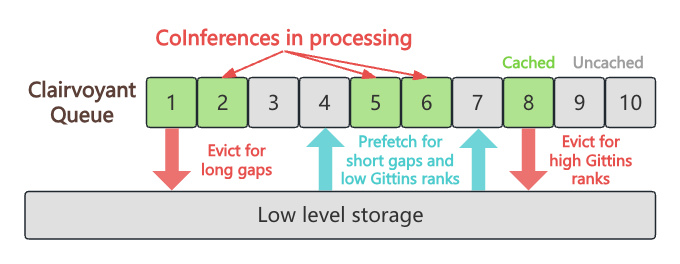
\includegraphics[width=1\linewidth]{figures/ClairvoyantQueue.png}
%     \caption{Illustration of resource eviction and prefetching between high and low-level storage using the Clairvoyant Queue.}
%     \label{fig:ClairvoyantQueue}
% \end{figure}





\subsubsection{Clairvoyant Queuing on Non-LLM Backends}
\label{subsubsec:queuing}
Serving LLM applications often requires diverse non-LLM bankends, the demands of which, as elaborated in \S\ref{subsec:demand_modeling}, are included in coinference modeling.
In production clusters concurrently serving massive LLM applications, it is possible that resource contention occurs on such non-LLM backends.
To elaborate, we focus on three typical types of LLM tools\footnote{
    While we pick up three relatively-simple tools for study in this part, we note that the general principle here can be applied to other professional tools, like the traditional symbolic solver used in AlphaGeometry~\cite{AlphaGeometry}.
}
(here we use a broad sense of \emph{tools} which refer to all the non-LLM components of LLM applications).
First, some code-writing applications~\cite{factool_code} may periodically verify the correctness of the generated code with a docker container (for better environment isolation); under insufficient CPU resources, the container launching requests would be queued on the scheduler. 
Second, LLM applications with RAG (like KBQAV~\cite{factool_kbqa}) may periodically search for documents from the websites, which, under limited network bandwidth, may cause non-negligible network queuing delay.
Third, LLM applications like HuggingGPT~\cite{hugginggpt} may call small models (hosted on dedicated GPU servers); facing bursting requests, such small models (constrained by the resources on the dedicated GPU servers) can also become a bottleneck. 

Note that our previous coinference scheduling priority is imposed to the LLM backends, and the above non-LLM tasks submitted to other backends are often handled by independent schedulers. % respectively managing each resource backend. 
For example, the docker launching requests would be submitted to a kubernetes scheduler.
Under the default strategy (e.g., FCFS) of those schedulers, it is possible that the non-LLM tasks of a high-priority application be queued for a long time, postponing the ultimate application completion.
To address this issue, we propose \emph{clairvoyant queuing on non-LLM backends}, which propagates the application priority to all the involved schedulers managing non-LLM backends.
This way, it can be ensured that both the LLM and non-LLM components of a high-priority application can be serviced without any queuing delay. 

% Non-LLM tasks also play a significant role in the inference processes of many applications. For instance, in certain code-writing applications~\cite{}, the system needs to verify the correctness of code generated by LLMs within a Docker container. Limited CPU resource makes a competition in creating containers. Additionally, in applications like KBQA~\cite{}, the system needs to search for information from websites, which, in environments with limited network resources, can lead to further competition. Moreover, applications such as HuggingGPT~\cite{} include DNN execution tasks that require GPU resources, creating yet another layer of competition. Resource contention causes these non-LLM tasks to wait for resources, potentially leading to higher-priority applications being blocked by lower-priority ones under the default FCFS scheduling strategy. To address this issue, we propagate the application’s priority to the non-LLM task execution manager, ensuring that tasks associated with higher-priority inferences are given precedence.


\subsubsection{Clairvoyant Backend Selection}
\label{subsubsec:selection}
So far, we focus on the cases with uniform LLM backends.
In practice, it is possible that the LLM service providers provision multiple backends each with distinct configurations~\cite{lin2024parrot}. % superiority.
For example, inference batch size is a critical hyperparameter that affects the latency-throughput trade-off: setting a larger batching size can yield a higher throughput (by 8.2$\times$) but the latency would also be higher (by $95\%$)~\cite{chen2023dissecting}.
For fast serving of LLM applications, we thus also need to properly select the backend for each stage based on its demand characteristics.

To address that problem, we can employ a heuristic, clairvoyant backend selection, which leverages our coinference demand information to judge backend suitability for each stage. 
Suppose there is a latency-sensitive backend (with batch size $B_\text{min}$) and a throughput-sensitive backend to choose---emulating a ``power-of-two-choices" scheduling space~\cite{sitaraman2001power}; given a stage, we schedule it to the latency-sensitive backend if its request parallelism is larger than $B\text{min}$, and otherwise to the throughput-sensitive backend, so as to attain fast stage completion. 
Our evaluations show that this heuristic can indeed work well in practice.
We note that the principle of clairvoyant backend selection can be extended to other multi-backend cases. 
For example, a cluster may have GPU nodes of different generations (with heterogeneous computation-memory ratios); based on the predicted request output length, we can schedule the (memory-intensive) long-output requests onto the backends with smaller computation-memory ratio (and vice versa), which can improve the overall resource utilization.


% In decoding processes characterized by low computation density, increasing the number of concurrent requests can significantly  improve resource utilization and overall throughput. However, this approach inevitably leads to increased latency for individual requests. Additionally, larger batch sizes require more GPU memory to store the KV Cache of active requests. To address this issue, service providers often deploy multiple backends with varied configurations to meet different SLOs. 
% Specifically, they configure backends with smaller batch sizes on GPUs with limited memory to cater to low-latency demands while saving costs, alongside backends with larger batch sizes to maximize throughput.

% Leveraging our coinference modeling, we can dynamically assess the number of concurrent requests within a coinference stage and intelligently route them to the most appropriate backend. For instance, in a map-reduce summarization application, map requests—which benefit from higher throughput—can be routed to backends with large batch sizes, thereby reducing stage latency. Conversely, single reduce requests, which require lower latency, will be directed to backends with smaller batch sizes, ensuring minimal request latency. This strategic routing optimizes the latency at each stage, thereby optimizing the latency of the entire application.
